\documentclass[anon]{CI}
\usepackage[latin1]{inputenc}
\usepackage[english]{babel}
\usepackage[]{algorithm2e}
\usepackage{graphicx}
% The following packages will be automatically loaded:
% amsmath, amssymb, natbib, graphicx, url, algorithm2e

\title[CI Project]{Swarm intelligence for counting the degrees of separation in Social Networks}

 % Use \Name{Author Name} to specify the name.
 % If the surname contains spaces, enclose the surname
 % in braces, e.g. \Name{John {Smith Jones}} similarly
 % if the name has a "von" part, e.g \Name{Jane {de Winter}}.
 % If the first letter in the forenames is a diacritic
 % enclose the diacritic in braces, e.g. \Name{{\'E}louise Smith}

 % Two authors with the same address
  % \coltauthor{\Name{Author Name1} \Email{abc@sample.com}\and
  %  \Name{Author Name2} \Email{xyz@sample.com}\\
  %  \addr Address}

 % Three or more authors with the same address:
 % \coltauthor{\Name{Author Name1} \Email{an1@sample.com}\\
 %  \Name{Author Name2} \Email{an2@sample.com}\\
 %  \Name{Author Name3} \Email{an3@sample.com}\\
 %  \addr Address}


 % Authors with different addresses:
 \author{\Name{�lex Pardo} \Email{alexpardo.5@gmail.com}\\
 \AND
 \Name{David S�nchez} \Email{sdividis@gmail.com}\\
 }

\begin{document}

\maketitle

\begin{abstract}
The six degrees of separation is a well-known properties of small world networks. Social networks are small-world ones and also have this property. We pretend to calculate the degrees on separations in some social networks. There is a large number of algorithms to obtain the shortest path between two nodes in a graph, which is the problem we need to solve in order to check de degrees of some datasets.
We would use Ant Colony Optimization (ACO) to solve the shortest path problem in a sub-optimal way. This Swarm Intelligent algorithm will help to solve a problem that is computationally hard when the number of edges and nodes increases. This Computational Intelligent algorithm is inspired in the behaviour of ants.

The next project try to join these two concepts: the six degree of separation as a Ant Colony Optimization problem in one. We will code the algorithm and see how this algorithm works in two socials networks like Twitter and BlogCatalog.

\end{abstract}

\begin{keywords}
Swarm Intelligence, Ant Colony Optimization, Twitter, , BlogCatalog, Degrees of Separation
\end{keywords}


\section{Problem statement and goals} % 1 p�gina

%\textbf{This is where the content of your paper starts. Remember:
%\begin{itemize}
%\item Limit the main text (without bibliography and appendices) to 10 pages.
%\item Include, either in the main text or the appendices, enough details to convince the lecturers of the project's merits.
%\item You should cite all relevant references, including your own.
%\end{itemize}}
\par
One of the most important features of humans and in general, of lots of animals, is the sociability. The ability of communicating each other in order to share knowledge. Human social relationships form a network where everyone is connected with those that communicates often (considered as friends). 
\\ \par
The theory of the six degrees of separation was originally set out by Frigyes Karinthy \citep{karinthy1929chain} and explains that everyone is connected to any other person in the world by six degrees. That means, if you want to met someone in the world, you will need to pass by other five persons, as maximum, between you and your objective so the last one will be the one you are trying to reach. During these last decades, the six degree theory has been used in many fields like economy, social networks and markets and is a known property of small-world networks where most nodes are not neighbours of one another, but most nodes can be reached from every other by a small number of steps.
\\\par
Twitter is one of the biggest social networks, that is over 200 million users and over 400 million tweets (the 140 character messages that are the main feature of this social network) every day \footnote{Information by March of 2013: \href{https://blog.twitter.com/2013/celebrating-twitter7}{https://blog.twitter.com/2013/celebrating-twitter7}}. The main idea is to create shorts messages of the 140 characters in order to express your ideas or opinions in a shorten way. Moreover, Twitter have introduced some concepts that are very popular now such as the \emph{hash-tag} which is a way of tagging the messages i order to find all the related ones.

%Another famous social network is Foursquare, a social network related to places in which you activate the application and notifies your friends that you have been in that place. The most active users in one place achieve some goals such as being the ``major'' of a certain place. Foursquare has over 45 million users and over 3 billion check-ins every day \footnote{Information by January of 2014: \href{https://foursquare.com/about}{https://foursquare.com/about}}.
We also used another dataset acquired from BlogCatalog, a social blog directory which manages the bloggers and their blogs. In this case, the edges are the friendships among the bloggers. The dataset we have has 10K nodes and over 300K edges and is available on \citep{ZafaraniLiu}.
\\\par
The main objective of this work will be to estimate the degrees of separation in BlogCatalog and if it is computationally possible, in Twitter and see if it is possible to obtain six degrees of separation between two random people. In order to do this task, it will use some ideas of the Computational Intelligence like Swarm Intelligence. In particular we are going to use Ant Colony Optimization (ACO) \citep{Colorni91} for Shortest Path finding (SPACO) \citep{angus}.



%Content:
%\begin{enumerate}
%\item Explain theory of the 6 degrees
%\item Define the network
%\item Goals: estimate the degrees of separation in twitter
%\end{enumerate}



\section{Previous work} % 2 p�gines


Ant Colony Optimization (ACO) was first introduced by Alberto Colorni \citep{Colorni91} in 1991. It was initially used for achieving a sub-optimal solution for the Traveling Salesman Problem (TSP). This algorithm has been used also for obtaining the shortest path between two nodes or points as is explained by Daniel Angus \citep{angus}.

Additionally, the theory of the six degrees of distance in Small World networks has been developed by Frigyes Karinthy \citep{karinthy1929chain} and it is also explained by Duncan Watts \citep{watts}.

Additionally, this theory has been used on social networks such as Twitter in which five degrees of separation has been demonstrated \citep{cheng}.

\section{The CI methods} % 3-4 p�gines

Swarm intelligence is a natural method based in the behaviour of decentralized individuals who obtain solutions for a certain problem taking profit of their interactions. These agents normally are simple, with a few capabilities and follow simple rules. It includes algorithms as ACO, flocking of the birds or bacterial grow among others. 
\\\\
As it is mentioned previously, we will use the ACO algorithm in order to obtain the degree of separation between two random people in a graph. This algorithm is inspired in the way ants have to solve the problem of finding the best path to achieve a goal such as going from the nest to the found food. Ants use the trace of pheromone as a guidance system in order to choose which path to follow. When an ant travels through two points it leaves a few of pheromone on the trail. The other ants around feel the pheromone and try to follow this path. The paths with few pheromone will have less probability than a path with higher amount of pheromone. As it is shown in Figure \ref{fig:aco}, the path of the ants converge to the shortest path between two points and this is the main feature of this method. We will use this idea of the shortest path between two points, as a minimum degree between two person in BlogCatalong and Twitter networks. In the appendix \ref{implementation}, it will be shown how the algorithm works.

\begin{figure}[htb!]
\centering
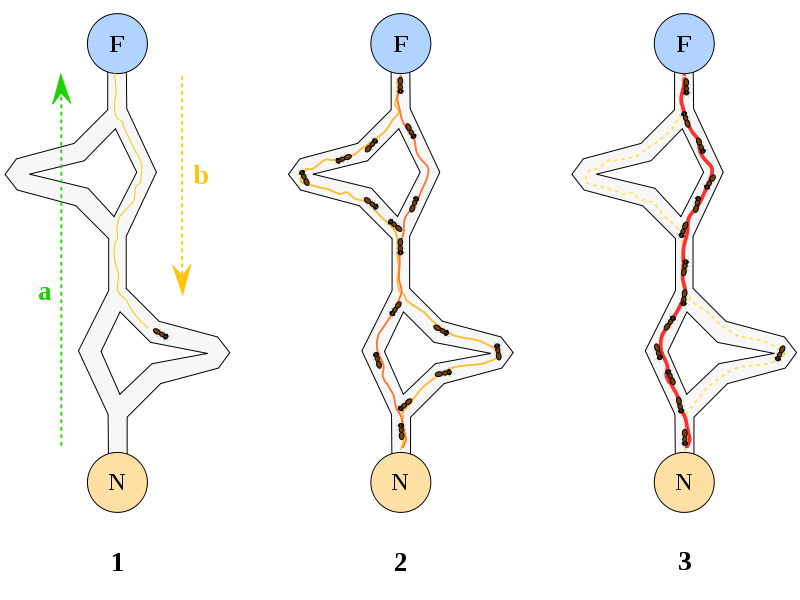
\includegraphics[scale = 0.4]{img/aco}
\caption[ACO algorithm]{ACO algorithm\protect\footnote{Credits to Johann Dr�o, 27 may 2006}}
\label{fig:aco}
\end{figure}

Some considerations needed to take into account are the parameters of the algorithm. These are: the amount of pheromone leaved by each ant, the number of ants of the system, the dissipation of the pheromone and the number of epochs the algorithm will run.

The amount of pheromone an ant leaves in the trail is has been fixed to one. Since the graph we are going is has not weighted edges (i.e. edges initially have weight 1), the pheromone leaved is always the same.
Those ants that have reached the objective node, return to the nest (starting node) and leave pheromone on the same path they followed to arrive to the objective.
Additionally as \citep{dorigo1999ant} recommends, the amount of pheromone of the system is kept fixed, so at each iteration it is normalized to always sum a value equal to the number of nodes.
% Amount of pheromone
% - set to 1
% - since weights are always 1, the pheromone is always the same
% - ants returning to the nest (start) leave pheromone also in the trail
% - additionally as \citep{dorigo1999ant} says, the amount of pheromone of the system is kept fixed, so at each iteration it is normalized to always sum a value equal to the number of nodes.

On each epoch, a fixed number of ants is introduced in the system so new ants can follow the paths started by other ants and discover another ones. This way we are assuring exploration over exploitation. We would prefer some short path from start to objective rather than one single path since, having a larger number of paths will increase the probability of finding the shortest path.
In order to optimize the algorithm, since we are trying to find a path shortest than 10 units of distance (it should be shortest than 7 but we allow paths a bit larger) those ants which are at distance 15 far from the nest are considered lost and are deleted from the system. This will increase the performance of the system.
% Number of ants in the system
% - on each epoch, some ants are introduced on the system this allows the new ants to follow the paths started by the ants on the previous epochs
% - Once an ant is at distance 15 from the nest, we consider the ant has been lost so we do not follow it anymore (i.e. the ant is deleted from the system) this allows the code to run much more faster since we are only interested in shortest paths.

Dissipation of pheromone allows the system to forget bad solutions. In essence, bad solutions are long so the ants take longer to go from the nest to the food, the dissipation allows the ants to explore additional paths. Shortest paths also suffer the dissipation but since are shorter, ants will arrive faster and the dissipation will be lower because ants will take less time in going to the objective and returning to the nest.

% Dissipation of the pheromone
% - disipation of pheromone allows the system to forget bad solutions in essence, bad solutions are long so the ants take longer to go from the nest to the food, the disipation allows the ants to explore aditional paths. Shortest paths also suffer the disipation but since are shorter, ants will arrive faster and the disipation will be compensated by the pheromone leaved

The number of epochs has to be taken into account using the number of ants on the system, the expected length of the path and the computational time associated to the problem.
If there are a large number of ants the system will converge earlier (due to the possibility of finding the path). A smaller number of ants will require to increase the number of epochs needed to converge.

% Number of epochs
% - the number of epochs has to be taken into account using the number of ants on the system, the expected lentgh of the path and the computational time associated to the problem.
% - num of ants -> if there are a lot of ants, the system will be slower but will converge earlier, if the number of ants is lower, we will have to increase the number of epochs in order to converge
% - expected length of the path -> the number of epochs is expected to be greatest than the expected length of the shortest path since ants perform one step at each epoch.
% - Computational time -> since we are working with huge graphs (3 million of nodes and 11 million of edges), the computational cost of the algorithm is crucial, and the greatest the number of epochs, the greatests the number of expaned nodes. As explained on \ref{implementation}, the pheromones saved are the ones in which the amount is increased, so when the number of expanded nodes increasesm the ammount of memory needed also increases.

\section{Results and Discussion} % 1-2 p�gines de text



In order to perform the tests we used three different datasets. The first ones are a subset of Twitter network. The third one has been obtained from \citep{ZafaraniLiu} and is based on BlogCatalog network. The acquisition of the Twitter graphs is explained in \ref{implementation}.
\par
Each dataset has been used changing the parameters of the algorithm in order to get the shortest path using the less computational resources. This parameters have been experimentally set.
On each execution, the starting and objective points are taken randomly from the whole graph.


\begin{figure}[htb!]
\centering     
\subfigure[First Twitter graph]{\label{fig:graph1}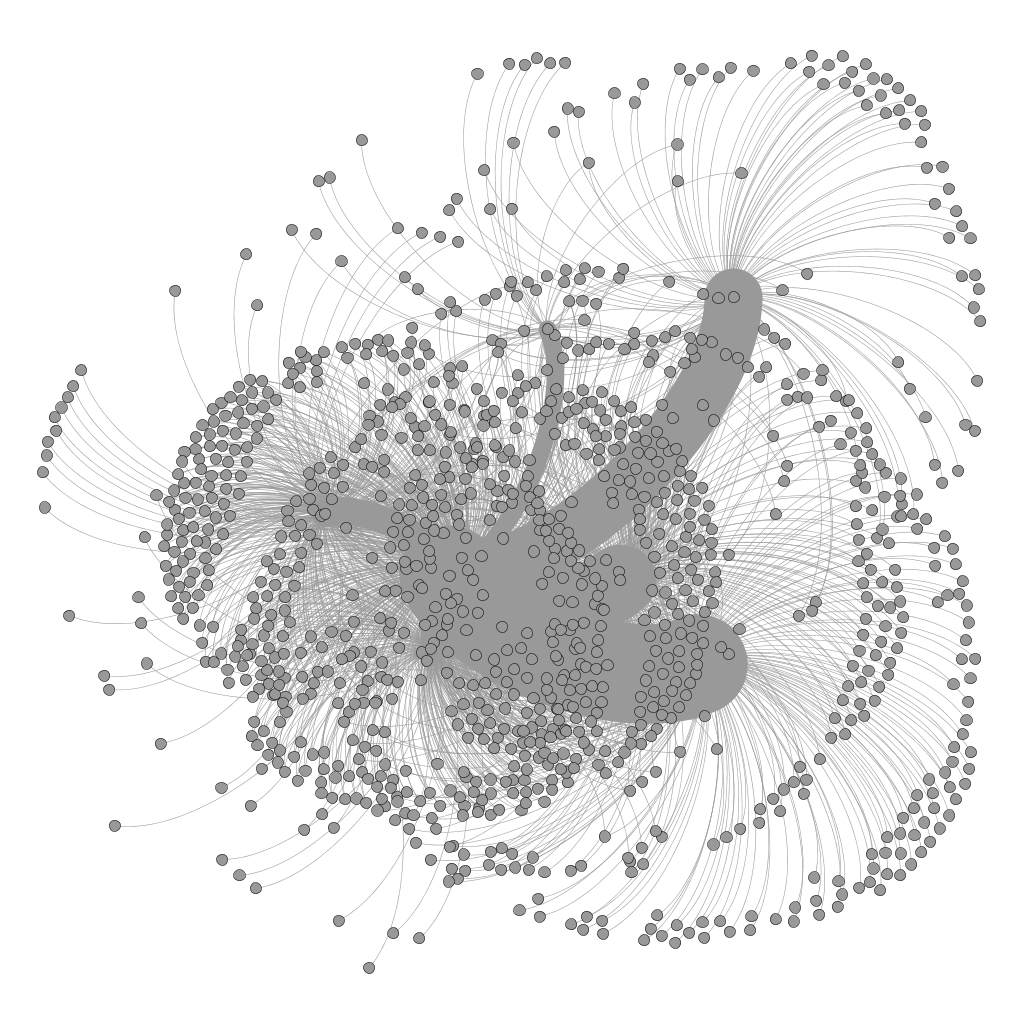
\includegraphics[width=60mm]{img/m1}}
\subfigure[Second Twitter Graph]{\label{fig:graph2}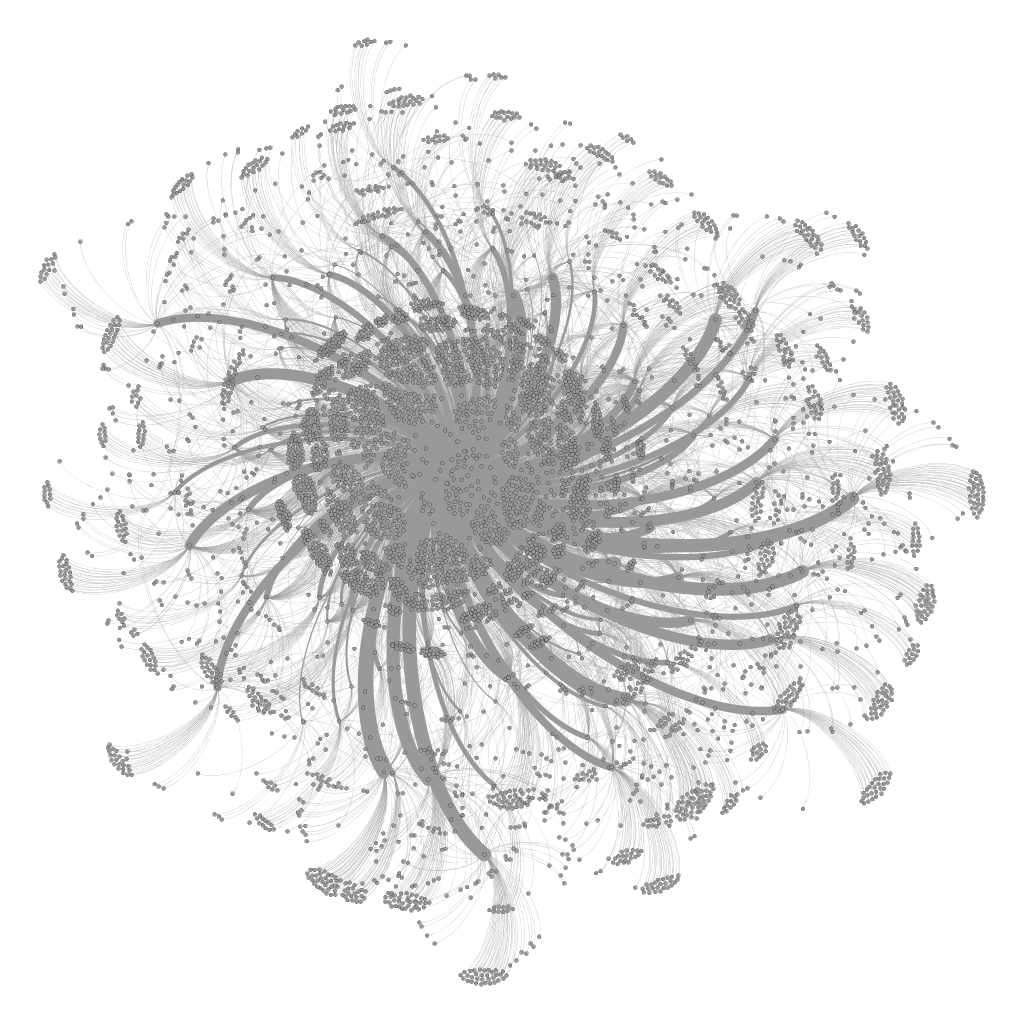
\includegraphics[width=60mm]{img/m2}}\\
\subfigure[BlogCatalog graph]{\label{fig:graph3}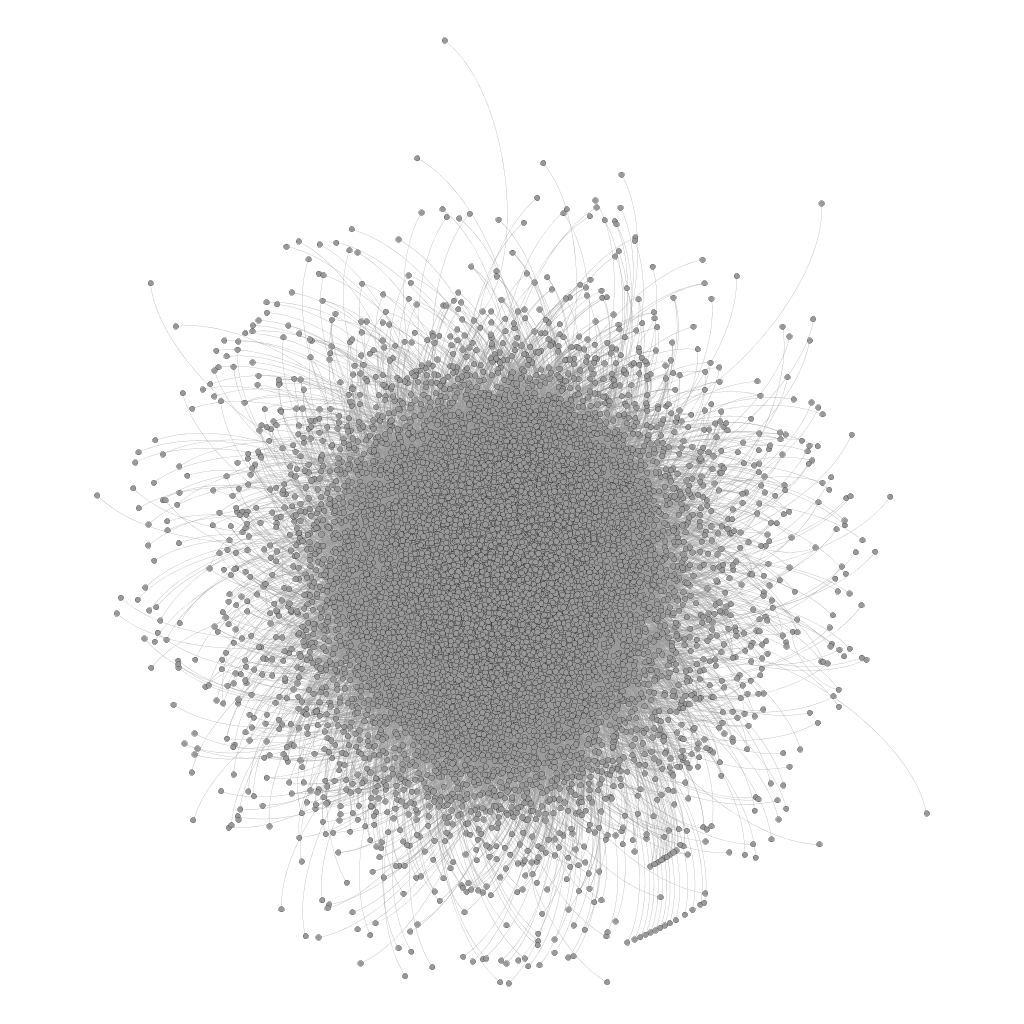
\includegraphics[width=60mm]{img/big}}\\
\caption{Plot of the datasets used}
\end{figure}



\begin{table}
\centering
\begin{tabular}{l|l}
\hline
NUM\_ANTS & Maximum number of the ants in the system \\ \hline
ITERATIONS & Number of the experiments \\ \hline
DECAY & Factor of evaporation of the pheromones \\ \hline
INCREMENT & Number of the increment of the pheromones \\ \hline
ANTS\_PER\_TURN & Number of ants at each turn that appears \\ \hline
MAX\_EPOCH & Number of the iterations at each experiment \\ \hline
\end{tabular}
\caption{Table of the parameters description of the algorithm}
\label{parameters}
\end{table}

The next Table \ref{datasets}, shows the number of the nodes and edges at each dataset.
\begin{table}[htb!]
\centering
\begin{tabular}{l|c|c}
~ & Number of nodes & Number of edges \\ \hline
Twitter(1) & 1146 & 1221 \\ 
Twitter(2) & 5691 & 6220 \\ 
BlogCatalog & 10312 & 333983 \\ \hline
\end{tabular}
\caption{Table of the experimental dataset}
\label{datasets}
\end{table}


\subsection{First dataset}

In Figure \ref{fig:graph1},one can see the graph plotted.


The parameters used for this graph are: 
\begin{itemize}
\item 10 Iterations
\item Increment of pheromone = 1
\item Decay of pheromone = 0.2
\item 3 ants introduced on each epoch
\item Maximum of 1000 epochs
\end{itemize}

In Table \ref{table:graph1} the results obtained are showed. Finally, the \textbf{mean of the shortest path is 6.2} with standard deviation of 2.74.

\begin{table}[htb!]
\centering
\begin{tabular}{c|c|c}
Execution	&	Shortest path	& Average path	\\ \hline
1			&	3				& 	7.23			\\
2			&	7				& 	7			\\
3			&	3				& 	8			\\
4			&	3				& 	7.28			\\
5			&	10				& 	14			\\
6			&	8				& 	8			\\
7			&	7				& 	7.56			\\
8			&	5				& 	5			\\
9			&	11				& 	11			\\
10			&	5				& 	9.6			\\
\end{tabular}
\caption{Results of the first graph}
\label{table:graph1}
\end{table}

\subsection{Second dataset}

In Figure \ref{fig:graph2}, one can see the graph plotted.


The parameters used for this graph are: 
\begin{itemize}
\item 10 Iterations
\item Increment of pheromone = 1
\item Decay of pheromone = 0.01
\item 5 ants introduced on each epoch
\item Maximum of 500 epochs
\end{itemize}

In Table \ref{table:graph2} the results obtained are showed. Finally, the \textbf{mean of the shortest path is 7.5} with standard deviation of 2.7.

\begin{table}[htb!]
\centering
\begin{tabular}{c|c|c}
Execution	&	Shortest path	& Average path	\\ \hline
1			&	5				& 	10.17		\\
2			&	3				& 	8.61			\\
3			&	4				& 	10.23		\\
4			&	11				& 	12.5			\\
5			&	9				& 	9			\\
6			&	8				& 	10			\\
7			&	9				& 	9			\\
8			&	11				& 	12.46		\\
9			&	6				& 	6			\\
10			&	9				& 	9			\\
\end{tabular}
\caption{Results of the second graph}
\label{table:graph2}
\end{table}

\subsection{Third dataset}

In Figure \ref{fig:graph3}, one can see the graph plotted.


The parameters used for this graph are: 
\begin{itemize}
\item 10 Iterations
\item Increment of pheromone = 1
\item Decay of pheromone = 0.01
\item 50 ants introduced on each epoch
\item Maximum of 300 epochs
\end{itemize}

In Table \ref{table:graph3} the results obtained are showed. Finally, the \textbf{mean of the shortest path is 7} with standard deviation of 3.06.

\begin{table}[htb!]
\centering
\begin{tabular}{c|c|c}
Execution	&	Shortest path	& Average path	\\ \hline
1			&	4				& 	8			\\
2			&	5				& 	5			\\
3			&	14				& 	14			\\
4			&	6				& 	9			\\
5			&	5				& 	5			\\
6			&	9				& 	9			\\
7			&	4				& 	4			\\
8			&	10				& 	10			\\
9			&	8				& 	10.5			\\
10			&	5				& 	5			\\
\end{tabular}
\caption{Results of the third graph}
\label{table:graph3}
\end{table}

\subsection{Discussion of the results}
The different tables of results Tables \ref{table:graph1}, \ref{table:graph2} and \ref{table:graph3} show several executions in order to get more realistic results. The parameters of the execution change between the different dataset in order to get better results depending on the features of each one (i.e. the number of nodes and edges). For example, the number of the ants that the algorithm introduces at each turn depends on the size of the graph (the higher the number of nodes, the higher the number of neighbours) so it is increased on bigger graphs.
\\\par
In Table \ref{table:graph1} we obtained the shortest path between the different execution between three and eleven having a mean of 6.2. The result is pretty good because it is very close to the value we are trying to obtain (six). Although the mean are 6.2, we obtained in three times that the shortest path are three. That is because, first of all we have an incomplete graph (Twitter is much more larger) and second, not all the nodes in a social network will have the same degree to every node, six (or five in the case of Twitter) is expected to be the mean distance.
\\\par
With the second dataset, we obtained worst results than the previous one. As Table \ref{table:graph2} shows, the shortest path of the different executions are between three and eleven as the first dataset. However, we obtained a mean of 7.5. This result is larger than six, the average path in the majority of the executions is higher than in the first graph. This second dataset is a bigger one. The increment of the nodes and edges has a negative effect in this case and we have tried to correct this effect adding more ants at each turn, decreasing the pheromone decay and increasing epochs though we did not obtain as good results as on the first Twitter dataset. The possible explanation is the construction of the dataset.
\\\par
Third dataset represents the BlogCatalog friendship network. The idea is the same, the nodes are bloggers and the edges are the connection between these people. As Table \ref{table:graph3} shows, the shortest path in all executions is between four and fourteen. These results are worst than the second dataset although the mean shortest graph is lower but with higher variance. So, although in this case we do not obtain the best shortest path we expected, the mean average shortest path is 7. The high variance is saying that the ants are finding much more larger distances in the graph. This could be a feature of this social network. As it is said before, the length of the shortest path is expected to have a mean of six. More executions and a higher number of ants is required in order to achieve more significant results. It could not be done due to computational limitations.

All the datasets have similar standard deviation and exist few variation or dispersion from the average results. Remember that a low standard deviation means that the data points tend to be very close to the expected value or mean. Although the variation is low, taking into account the desired results (values close or lower than six) in some cases is too high (a distance of fourteen is too high). As it is said on the discussion of the results achieved on the third dataset, the number of executions should be higher and also the number of ants in order to have less bias on the results and increase the probability of achieving the shortest path.

Finally, we think that the selection of the parameters is very important since it has a high impact on the results. As there is no metric for setting them, they have to be experimentally set.

\section{Extensions, strengths and weaknesses}

Initially, we expected to use a huge Twitter dataset (over 85 million edges and 11 million nodes) and a smaller one of Foursquare (another social network). This graphs were computationally intractable since not only the number of nodes and edges is increased, but also the number of ants required to find the path and therefore the pheromone matrix.
It would be very interesting to execute this code in these big datasets which contain millions of nodes. It is not that easy to find big social network datasets on the Internet. However, with the small dataset used, we obtained good results and the method has been proved to work pretty well. So, we think that the algorithm also should obtain good results in this large datasets but we cannot ensure it by now.

Other extension can be introducing more ants in the system. The number of the ants can be proportional to the size of the dataset and the large datasets can use more ants than the smaller ones. We could compare the influence of this parameter depending on the size of the dataset and estimate the more suitable value for each problem.

One of the strengths of this method is the optimization performed in order to have less computational cost and be able to run it (without parallelized code) in a laptop using a relatively big dataset. 
ACO method allows a fast near-optimal result of the shortest path in huge graphs having an easy implementation and a simple theory behind it.

One of the weakness is that the method is not replicable, that is, every execution could have a different result, for this reason it is mandatory to execute the algorithm several times. Due to computational cost, we were not able to perform as many tests as we expected, for example, compare the parameters used or have a large number of executions in order to have a better approximation of the real mean path of the graphs.

\section{Conclusions}
Ant Colony Optimization is an easy way of finding the shortest path in those environments in where an optimal solution is impossible to achieve. In our specific problem of obtaining the degrees of separation between random people in social networks, the algorithm performed well and the results obtained were close to the ones expected.

Due to computational requirements of the algorithm we were not able to perform the tests on the desired datasets but we solved it using smaller ones but yet extracted from real social networks.

The theory behind the small world networks is really surprising and interesting and have some nice properties that could be exploited in a variety of areas such as predicting the extension of a rumor or in order to predict the impact of performing a commercial campaign in a certain social network.

Finally, the algorithm performed as expected, we have used some of the tricks present on literature in order to make the method perform better and the final results are good and are the ones we expected to achieve. It would be interesting to apply the algorithm to a huge social network such as Twitter or Facebook which are the most common nowadays.

\vspace{1cm}
\bibliography{bibliography.bib}

\appendix


\section{Implementation details} 
\label{implementation}

The application has been coded using Python 2.7.6 \footnote{Python webpage: http://www.python.org/}. The system uses NetworkX \citep{networkx} library in order to represent the graph. Additionally, in order to create an small dataset based on twitter, we used Twython implementation of the Twitter API in order to acquire the data and again, NetworkX in order to save the resulting graph. Also we use the matplotlib library in order to plot the graphs \citep{matplotlib}.

\subsection{Dataset retrieval}

In order to create an small dataset based on Twitter, Twython (based on Twitter API) has been used.
Due to Twitter limitations (only five-teen queries every five-teen minutes), we were not able to obtain a really big graph. What has been done is, beginning from a certain user, keep expanding the neighbours. Using his method we obtained two different graphs, a bigger and an smaller one. This two graphs are the ones on the left in Figure \ref{fig:graphs}.
\subsection{Algorithm}

Here the pseudocode of ACO is presented. In Algorithm \ref{alg:main}, one can see the main loop of the method and in Algorithm \ref{alg:step}, the step performed by each ant. As could be seen, the algorithm is pretty simple.

\begin{algorithm}
 \KwResult{Obtain the shortest path in a graph}
 initialize $G:=$Graph, $P:=$Pheromone and $A:=$Ants \\
 \For{each epoch}{
 	\For{each $a \in A$}{
 		$a$.step($P$)\\
 		Save new pheromone into a tmp variable\\
 		\If{$a$ in objective}{
 			$a$.returnNest()\\
 		}
 	}
 	update $P$\\
 }
 Obtain the shortest path for each $a\in A$ that finished
 		
 \caption{Main function}
 \label{alg:main}
\end{algorithm}

\begin{algorithm}
\KwResult{The ant performs one step}
Find the neighbours in $G$\\
Get the pheromone on each edge\\
Get a random number using the pheromone as probabilities\\
Move towards the selected edge\\
Leave pheromone\\
\caption{Ant step}
\label{alg:step}
\end{algorithm}

Next, some details of the implementation are explained:

\begin{itemize}
\item \textbf{Ants}: An ant class is defined in order to encapsulate all the concepts, methods and variables of the ant. As internal attributes, this class has the path, the starting point, the final point and the increment of the pheromones at each step. The class also has some methods in order to make the ants to perform a certain task. This methods are setStart(), setObjective(), step(), chooseNeighbour(), hasReachedObjective() and returnToStart().

%\item \textbf{Pheromone}: The pheromone is the most important part of othe problem. Ants try to follow the path which contains a higher amount of pheromone. However the pheromone effect disappears with the time (it evaporates). For this reason, in the algorithm, two parameters need to be defined in order to determine the quantity of pheromone that leaves the ant and the quantity of pheromone evaporated at each turn. 

\item \textbf{Choice the edge}: Every ant has to select one edge at each step. This is done using the pheromone as a probability of choosing that edge. This is done by normalizing the pheromone in order to sum one and then a random number is used to select the chosen path. It is performed like in a roulette wheel, where each edge has a bigger or smaller slice of the wheel so it has more or less probability.

\item \textbf{Start and final points of the ants}: The algorithm selects always randomly the start and the final point of the ants using the standard random methods of the python library.

\item \textbf{Ants at each turn}: The algorithm does not start with all the ants in the start point. At each turn, the algorithm adds more ants placed in the starting point. Also, we add a parameter named \emph{NUM\_ANTS} to control the maximum number of the ants in the whole system.

\end{itemize}



\end{document}
